%-----------------------------------------------------------------------------------------------------------------------------------------------%
%	The MIT License (MIT)
%
%	Copyright (c) 2019 Jan Küster
%
%	Permission is hereby granted, free of charge, to any person obtaining a copy
%	of this software and associated documentation files (the "Software"), to deal
%	in the Software without restriction, including without limitation the rights
%	to use, copy, modify, merge, publish, distribute, sublicense, and/or sell
%	copies of the Software, and to permit persons to whom the Software is
%	furnished to do so, subject to the following conditions:
%	
%	THE SOFTWARE IS PROVIDED "AS IS", WITHOUT WARRANTY OF ANY KIND, EXPRESS OR
%	IMPLIED, INCLUDING BUT NOT LIMITED TO THE WARRANTIES OF MERCHANTABILITY,
%	FITNESS FOR A PARTICULAR PURPOSE AND NONINFRINGEMENT. IN NO EVENT SHALL THE
%	AUTHORS OR COPYRIGHT HOLDERS BE LIABLE FOR ANY CLAIM, DAMAGES OR OTHER
%	LIABILITY, WHETHER IN AN ACTION OF CONTRACT, TORT OR OTHERWISE, ARISING FROM,
%	OUT OF OR IN CONNECTION WITH THE SOFTWARE OR THE USE OR OTHER DEALINGS IN
%	THE SOFTWARE.
%	
%
%-----------------------------------------------------------------------------------------------------------------------------------------------%


%============================================================================%
%
%	DOCUMENT DEFINITION
%
%============================================================================%

%we use article class because we want to fully customize the page and don't use a cv template
\documentclass[10pt,A4]{article}	


%----------------------------------------------------------------------------------------
%	ENCODING
%----------------------------------------------------------------------------------------

% we use utf8 since we want to build from any machine
\usepackage[utf8]{inputenc}

%----------------------------------------------------------------------------------------
%	LOGIC
%----------------------------------------------------------------------------------------

% provides \isempty test
\usepackage{xstring, xifthen}

%----------------------------------------------------------------------------------------
%	FONT BASICS
%----------------------------------------------------------------------------------------

% some tex-live fonts - choose your own

%\usepackage[defaultsans]{droidsans}
%\usepackage[default]{comfortaa}
%\usepackage{cmbright}
\usepackage[default]{raleway}
%\usepackage{fetamont}
%\usepackage[default]{gillius}
%\usepackage[light,math]{iwona}
%\usepackage[thin]{roboto} 

% set font default
\renewcommand*\familydefault{\sfdefault} 	
\usepackage[T1]{fontenc}
\usepackage[italian]{babel}

% more font size definitions
\usepackage{moresize}

%----------------------------------------------------------------------------------------
%	FONT AWESOME ICONS
%---------------------------------------------------------------------------------------- 

% include the fontawesome icon set
\usepackage{fontawesome}

% use to vertically center content
% credits to: http://tex.stackexchange.com/questions/7219/how-to-vertically-center-two-images-next-to-each-other
\newcommand{\vcenteredinclude}[1]{\begingroup
\setbox0=\hbox{\includegraphics{#1}}%
\parbox{\wd0}{\box0}\endgroup}

% use to vertically center content
% credits to: http://tex.stackexchange.com/questions/7219/how-to-vertically-center-two-images-next-to-each-other
\newcommand*{\vcenteredhbox}[1]{\begingroup
\setbox0=\hbox{#1}\parbox{\wd0}{\box0}\endgroup}

% icon shortcut
\newcommand{\icon}[3] { 							
	\makebox(#2, #2){\textcolor{maincol}{\csname fa#1\endcsname}}
}	

% icon with text shortcut
\newcommand{\icontext}[4]{ 						
	\vcenteredhbox{\icon{#1}{#2}{#3}}  \hspace{2pt}  \parbox{0.9\mpwidth}{\textcolor{#4}{#3}}
}

% icon with website url
\newcommand{\iconhref}[5]{ 						
    \vcenteredhbox{\icon{#1}{#2}{#5}}  \hspace{2pt} \href{#4}{\textcolor{#5}{#3}}
}

% icon with email link
\newcommand{\iconemail}[5]{ 						
    \vcenteredhbox{\icon{#1}{#2}{#5}}  \hspace{2pt} \href{mailto:#4}{\textcolor{#5}{#3}}
}

%----------------------------------------------------------------------------------------
%	PAGE LAYOUT  DEFINITIONS
%----------------------------------------------------------------------------------------

% page outer frames (debug-only)
% \usepackage{showframe}		

% we use paracol to display breakable two columns
\usepackage{paracol}

% define page styles using geometry
\usepackage[a4paper]{geometry}

% remove all possible margins
\geometry{top=1cm, bottom=1cm, left=1cm, right=1cm}

% microtipografia: meno righe che sforano nel PDF
\usepackage{microtype}
% un po' più di tolleranza sullo spazio inter-parola nelle colonne strette
\setlength{\emergencystretch}{2.5em}

\usepackage{fancyhdr}
\pagestyle{empty}

% space between header and content
% \setlength{\headheight}{0pt}

% indentation is zero
\setlength{\parindent}{0mm}

%----------------------------------------------------------------------------------------
%	TABLE /ARRAY DEFINITIONS
%---------------------------------------------------------------------------------------- 

% extended aligning of tabular cells
\usepackage{array}

% custom column right-align with fixed width
% use like p{size} but via x{size}
\newcolumntype{x}[1]{%
>{\raggedleft\hspace{0pt}}p{#1}}%


%----------------------------------------------------------------------------------------
%	GRAPHICS DEFINITIONS
%---------------------------------------------------------------------------------------- 

%for header image
\usepackage{graphicx}

% use this for floating figures
% \usepackage{wrapfig}
% \usepackage{float}
% \floatstyle{boxed} 
% \restylefloat{figure}

%for drawing graphics		
\usepackage{tikz}				
\usetikzlibrary{shapes, backgrounds,mindmap, trees}

%----------------------------------------------------------------------------------------
%	Color DEFINITIONS
%---------------------------------------------------------------------------------------- 
\usepackage{transparent}
\usepackage{color}

% primary color
\definecolor{maincol}{RGB}{ 223, 43, 43}
\definecolor{skillcol}{RGB}{ 223, 123, 123}
%\definecolor{maincol}{RGB}{0,128,0}

% accent color, secondary
% \definecolor{accentcol}{RGB}{ 250, 150, 10 }

% dark color
\definecolor{darkcol}{RGB}{ 70, 70, 70 }

% light color
\definecolor{lightcol}{RGB}{245,245,245}


% Package for links, must be the last package used
\usepackage[hidelinks]{hyperref}

% returns minipage width minus two times \fboxsep
% to keep padding included in width calculations
% can also be used for other boxes / environments
\newcommand{\mpwidth}{\linewidth-\fboxsep-\fboxsep}
	


%============================================================================%
%
%	CV COMMANDS
%
%============================================================================%

%----------------------------------------------------------------------------------------
%	 CV LIST
%----------------------------------------------------------------------------------------

% renders a standard latex list but abstracts away the environment definition (begin/end)
\newcommand{\cvlist}[1] {
  \begin{itemize}
    \setlength{\itemsep}{2pt} % Riduci lo spazio tra gli elementi
    \setlength{\topsep}{0pt} % Riduci lo spazio prima di un elemento
    #1
  \end{itemize}
}

%----------------------------------------------------------------------------------------
%	 CV TEXT
%----------------------------------------------------------------------------------------

% base class to wrap any text based stuff here. Renders like a paragraph.
% Allows complex commands to be passed, too.
% param 1: *any
\newcommand{\cvtext}[1] {
	\begin{tabular*}{1\mpwidth}{p{0.98\mpwidth}}
		\parbox{1\mpwidth}{#1}
	\end{tabular*}
}

%----------------------------------------------------------------------------------------
%	CV SECTION
%----------------------------------------------------------------------------------------

% Renders a a CV section headline with a nice underline in main color.
% param 1: section title
\newcommand{\cvsection}[1] {
	\vspace{14pt}
	\cvtext{
		\textbf{\LARGE{\textcolor{darkcol}{\uppercase{#1}}}}\\[-4pt]
		\textcolor{maincol}{ \rule{0.1\textwidth}{2pt} } \\
	}
}

%----------------------------------------------------------------------------------------
%	META SKILL
%----------------------------------------------------------------------------------------

% Renders a progress-bar to indicate a certain skill in percent.
% param 1: name of the skill / tech / etc.
% param 2: level (for example in years)
% param 3: percent, values range from 0 to 1
% Nome e barra nello stesso blocco (stesso layout del CV in inglese).
\newcommand{\cvskill}[3] {%
	\par\addvspace{4pt}%
	\noindent
	\begin{minipage}[t]{1\mpwidth}
		\textcolor{black}{\textbf{#1}}\\[-6pt]
		\hspace{4pt}%
		\begin{tikzpicture}[scale=1,rounded corners=2pt,very thin,baseline={(0,0.075)}]
			\fill [lightcol] (0,0) rectangle (1\mpwidth, 0.15);
			\fill [skillcol] (0,0) rectangle (#3\mpwidth, 0.15);
		\end{tikzpicture}%
	\end{minipage}%
	\par
}


%----------------------------------------------------------------------------------------
%	 CV EVENT
%----------------------------------------------------------------------------------------

\newcommand{\cvevent}[7] {
    \ifthenelse{\value{eventcount}>0}{\vspace{4pt} \noindent\textcolor{lightcol}{\rule{\linewidth}{0.5pt}} \vspace{10pt}}{}
    \stepcounter{eventcount}

    \parbox{\mpwidth}{
        \begin{tabular*}{1\mpwidth}{p{0.72\mpwidth} r}
            \raggedright\textcolor{black}{\textbf{#2}} & 
            \textbf{\underline{\textcolor{black}{#1}}} \\
            \raggedright\textcolor{maincol}{\textbf{#3}} & \\
        \end{tabular*}\\[6pt]

        \ifthenelse{\isempty{#4}}{}{
            \cvtext{#4}\\
        }
    }

    \ifthenelse{\isempty{#5}}{}{
        \vspace{4pt}
        {#5}
    }
    
    \parbox{\mpwidth}{
    \ifthenelse{\isempty{#6}}{}{
        \vspace{4pt}
        \cvtext{\textbf{Tecnologie:}}%\\
        {#6}
    }
    }

    \parbox{\mpwidth}{
    \ifthenelse{\isempty{#7}}{}{
        \vspace{4pt}
        \cvtext{\textbf{Risultati:}}%\\
        {#7}
    }
    }
    
    \vspace{4pt}
}

%----------------------------------------------------------------------------------------
%	 CV META EVENT
%----------------------------------------------------------------------------------------

% Renders a CV event on the sidebar
% param 1: title
% param 2: subtitle (optional)
% param 3: customer, employer, etc,. (optional)
% param 4: info text (optional)
\newcommand{\cvmetaevent}[4] {
	\textcolor{maincol} {\cvtext{\textbf{\begin{flushleft}#1\end{flushleft}}}}

	\ifthenelse{\isempty{#2}}{}{
	\textcolor{darkcol} {\cvtext{\textbf{#2}} }
	}

	\ifthenelse{\isempty{#3}}{}{
		\cvtext{{ \textcolor{darkcol} {#3} }}\\
	}

	\cvtext{#4}\\[14pt]
}

%---------------------------------------------------------------------------------------
%	QR CODE
%----------------------------------------------------------------------------------------

% Renders a qrcode image (centered, relative to the parentwidth)
% param 1: percent width, from 0 to 1
\newcommand{\cvqrcode}[1] {
	\begin{center}
		\includegraphics[width={#1}\mpwidth]{qrcode}
	\end{center}
}


%============================================================================%
%
%
%
%	DOCUMENT CONTENT
%
%
%
%============================================================================%
\begin{document}
\newcounter{eventcount}
\setcounter{eventcount}{0}
\columnratio{0.31}
\setlength{\columnsep}{2.2em}
\setlength{\columnseprule}{4pt}
\colseprulecolor{lightcol}
\begin{paracol}{2}
\begin{leftcolumn}
%---------------------------------------------------------------------------------------
%	META IMAGE
%----------------------------------------------------------------------------------------
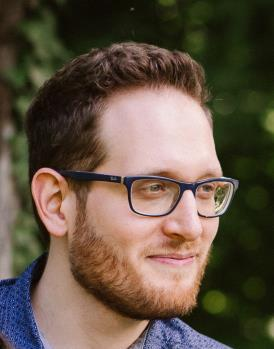
\includegraphics[width=\linewidth]{profile.jpg}	%trimming relative to image size

%---------------------------------------------------------------------------------------
%	CONTATTI (sotto la foto, prima delle competenze)
%---------------------------------------------------------------------------------------
\cvsection{CONTATTI}

\icontext{MapMarker}{12}{Avigliana (TO), Italia}{black}\\[4pt]
\icontext{MobilePhone}{12}{338-9904630}{black}\\[4pt]
\iconemail{Envelope}{12}{danieleb88@gmail.com}{danieleb88@gmail.com}{black}\\[4pt]
\iconhref{Github}{12}{github.com/dbortoluzzi}{https://github.com/dbortoluzzi}{black}\\[4pt]
%\iconhref{Orcid}{12}{0009-0004-2056-9111}{https://orcid.org/0009-0004-2056-9111}{black}\\[4pt]

\vspace{8pt}

%---------------------------------------------------------------------------------------
%	META SKILLS
%---------------------------------------------------------------------------------------
\cvsection{COMPETENZE}

\cvskill{Java} {10+ anni} {1.0}
\cvskill{Spring Framework} {10+ anni} {0.9}
\cvskill{Quarkus} {2+ anni} {0.8}
\cvskill{Scala} {5+ anni} {0.9}
\cvskill{Kubernetes} {4+ anni} {0.8}
\cvskill{AWS} {3+ anni} {0.75}
\cvskill{Terraform} {2+ anni} {0.75}
\cvskill{Linux} {10+ anni} {1.0}
\cvskill{Python} {5+ anni} {0.8}
\cvskill{TypeScript} {5+ anni} {0.8}
\cvskill{C++} {3+ anni} {0.8}
\cvskill{ROS2} {2+ anni} {0.7}

\vspace{8pt}
\cvskill{Lavoro di squadra} {10+ anni} {1.0}
\cvskill{Risoluzione di problemi} {10+ anni} {0.9}
\cvskill{Mentoring / tutoraggio} {10+ anni} {0.9}
\cvskill{Leadership di team} {5+ anni} {0.9}
\cvskill{Innovazione} {10+ anni} {0.9}
\cvskill{Capacità decisionale} {5+ anni} {0.8}
\cvskill{Comunicazione} {2+ anni} {0.8}
\cvskill{Negoziazione} {2+ anni} {0.6}

\vfill\null


%---------------------------------------------------------------------------------------
%	EDUCATION
%----------------------------------------------------------------------------------------
\newpage
\cvsection{ISTRUZIONE}

\cvmetaevent
{09/2013 -- 07/2022}
{Laurea Magistrale in Informatica (Livello 7 EQF)}
{Università di Torino}
{Voto di laurea: \emph{110/110 con lode e dignità di stampa}.}

\cvmetaevent
{09/2007 -- 06/2011}
{Laurea Triennale in Informatica (Livello 6 EQF)}
{Università Ca' Foscari di Venezia}
{Voto di laurea: \emph{104/110}.}

\cvmetaevent
{09/2002 -- 06/2007}
{Diploma di Liceo Scientifico}
{Liceo Scientifico Statale “G. Marconi” di Conegliano (TV)}
{Piano Nazionale per l'Informatica.\\
Voto finale: 90/100.}

\vfill\null

%---------------------------------------------------------------------------------------
%	PUBBLICAZIONI
%----------------------------------------------------------------------------------------

\cvsection{PUBBLICAZIONI}
% Stesso testo del CV in inglese: titoli e citazioni bibliografiche \emph{non} tradotti.

\cvtext{
\textbf{G. Audrito, A. Basso, D. Bortoluzzi, F. Damiani, G. Scarso, G. Torta.} \\
``Exploiting Aggregate Programming in a Multi-Robot Service Prototype'', \\
In: Proc.\ 17th Workshop on Programming Language Approaches to Concurrency and Communication-cEntric Software (PLACES~2026). \textit{Electronic Proceedings in Theoretical Computer Science} (EPTCS), vol.~444, 2026, pp.~45--57. \href{https://arxiv.org/abs/2604.06876}{arXiv:2604.06876}
}

\vspace{10pt}

\cvtext{
\textbf{G. Audrito, D. Bortoluzzi, F. Damiani, G. Scarso, G. Torta, A. Basso, M. Cochi, L. Gusman, L. Comba, P. Gay, P. Dal~Zovo, G. Galati, F. Gallo, A. Grdadolnik, M. Pescarollo, P. Pisano.} \\
``Lambdas at the Far Edge: a Tale of Flying Lambdas and Lambdas on Wheels'', \\
In: Logics and Type Theory (LTT~2026): essays dedicated to Stefano Berardi. \textit{Electronic Proceedings in Theoretical Computer Science} (EPTCS), vol.~441, 2026, pp.~19--45. \href{https://arxiv.org/abs/2603.04008}{arXiv:2603.04008}
}

\vspace{10pt}

\cvtext{
\textbf{Audrito, G., Bortoluzzi, D., Damiani, F., Scarso, G., Torta, G.} \\
"An Enhanced Exchange Operator for XC." In: Castellani, I., Tiezzi, F. (eds) Coordination Models and Languages. COORDINATION 2024. Lecture Notes in Computer Science, vol 14676. Springer, Cham
}

\vspace{10pt}

\cvtext{
\textbf{L. Nitti, D. Bortoluzzi, A. Biglia, D. Ricauda Aimomino, G. Torta, G. Audrito, F. Damiani, P. Gay. A.
Rapp, L. Comba.} \\
"UAS-swarm based surveillance system for UGVs safety functionality", Proc. of
the 15th European Conference on Precision Agriculture, 2024, Barcelona (Spain)
}

\vspace{10pt}

\cvtext{
\textbf{A. Basso, D. Bortoluzzi and G. Torta.} \\
"Implementation of an IoT Wearable Prototype on a Standard AI Architecture," 2022 IEEE Intl Conf on Dependable, Autonomic and Secure Computing, Intl Conf on Pervasive Intelligence and Computing, Intl Conf on Cloud and Big Data Computing, Intl Conf on Cyber Science and Technology Congress (DASC / PiCom / CBDCom / CyberSciTech), Falerna, Italy, 2022, pp. 1-5
}

\vspace{10pt}

\cvtext{
\textbf{A. Basso, D. Bortoluzzi, G.Torta, D. Pau, L. Chariglione, F. Damiani.} \\
"Architecture standardization for AI deployment on tiny micro-controllers", \\
Proc. of the 12th IEEE Int. Conf. on Consumer Technology, 2-6 September 2022, Berlin (Germany)
}

\vfill

\end{leftcolumn}
\begin{rightcolumn}

%---------------------------------------------------------------------------------------
%	TITOLO
%----------------------------------------------------------------------------------------
\fcolorbox{white}{darkcol}{\begin{minipage}[c][3.5cm][c]{1\mpwidth}
	\begin {center}
		\HUGE{ \textbf{ \textcolor{white}{ \uppercase{DANIELE BORTOLUZZI} } } } \\[-24pt]
		\textcolor{white}{ \rule{0.1\textwidth}{1.25pt} } \\[4pt]
		\large{ \textcolor{white} {Architetto Software e IoT / R\&D} }
	\end {center}
\end{minipage}} \\[14pt]
\vspace{-12pt}

%---------------------------------------------------------------------------------------
%	PROFILO
%----------------------------------------------------------------------------------------
\vspace{8pt}
\cvsection{PROFILO}

\cvtext{\textbf{15 anni} su progetti articolati---dalla definizione dell'architettura al rilascio in esercizio---con \emph{stack} cloud-native, piattaforme dati, intelligenza artificiale applicata, ambienti AWS e infrastruttura gestita con Terraform.\\ Ho ricoperto ruoli di referente tecnico, coordinamento del team, consegna \emph{chiavi in mano} e affiancamento costante a sviluppatori e committenti.\\[7pt]
Mi occupo anche di \textbf{docenza} su cloud e sistemi distribuiti: container, microservizi, Spring e Spring Cloud, Docker, Kubernetes e OpenStack, in master e percorsi con atenei e partner. In questo periodo insegno nel \href{https://www.mastercloudcomputing.it/}{Master in Cloud Computing} dell'\textbf{Università di Torino} con COREP; valuto altri incarini formativi (seminari, moduli, formazione in azienda) anche fuori da quel contesto.\\[7pt]
Affianco a questo una \textbf{ricerca} ancora operativa su swarm intelligence e IoT, con attività su \emph{rover}, \emph{droni} e sistemi \emph{embedded}, tra laboratorio e sperimentazione sul campo.}

%---------------------------------------------------------------------------------------
%	ESPERIENZA LAVORATIVA
%----------------------------------------------------------------------------------------
\vspace{16pt}
\cvsection{LAVORO}

\cvevent
{03/2025 -- oggi}
{Consulente IT freelance}
{Remoto, Torino}
{Consulente indipendente: \underline{architettura software}, \underline{consegna chiavi in mano}, coordinamento del team e \underline{mentoring} su piattaforme cloud-native, prodotti dati e soluzioni industriali con \underline{AI} (inclusa l'\underline{Agriculture~4.0}).}
{\cvlist{
	\item \underline{Architetture a microservizi} (servizi indipendenti con \underline{Quarkus}), interfacce \underline{React} che consumano le API, e integrazione tra componenti distribuiti.
	\item \underline{Pipeline di ingestion dati} e \underline{dashboard} per monitoraggio, esplorazione e uso operativo di grandi dataset.
	\item \underline{Deploy su AWS} e infrastruttura as code: provisioning di ambienti e macchine con \underline{Terraform}.
	\item Progetti di \underline{AI} per \underline{analisi dati} e \underline{computer vision} applicati a casi d'uso \underline{Agriculture~4.0}.
}}
{\cvlist{
	\item \underline{Quarkus}, \underline{React} (TypeScript), microservizi, \underline{Redis}, \underline{AWS}, \underline{Terraform}, Python (AI e dati).
}}
{\cvlist{
	\item \underline{Team leader}, \underline{architetto software} e ingegnere operativo in incarichi \underline{chiavi in mano}.
	\item \underline{Mentoring} di sviluppatori e team di progetto lungo tutto il ciclo: progettazione, implementazione e messa in produzione.
}}

\cvevent
{11/2025 -- 04/2026}
{Docente a contratto}
{COREP (Torino)}
{Didattica in presenza per il \href{https://www.mastercloudcomputing.it/}{Master in Cloud Computing} (IA e Internet delle cose), \underline{master universitario di I livello} dell'\underline{Università di Torino}, con COREP.}
{\cvlist{
	\item Corso tenuto: ``Containerization and Virtualization Platforms'' (piattaforme di containerizzazione e virtualizzazione).
	\item Argomenti trattati: \underline{Spring Boot}, \underline{microservizi}, \underline{Docker}, \underline{Kubernetes} e OpenStack.
}}
{\cvlist{
	\item \underline{Spring Boot}, microservizi, \underline{Docker}, \underline{Kubernetes}, OpenStack, Java.
}}
{}

\cvevent
{03/2023 -- 02/2025}
{Assegnista di ricerca}
{Università di Torino, Dipartimento di Informatica}
{Nel gruppo MoVeRe dell'Università di Torino conduco ricerca sul paradigma di \underline{Programmazione aggregata}, per la \underline{coordinazione} tra entità eterogenee.}
{\cvlist{
	\item Partecipazione al progetto PRIN 2020 \underline{COMMON-WEARS}.
	\item Collaborazione su verticalizzazioni e PoC in \underline{Smart Mobility} e \underline{Industria 4.0}.
	\item Supporto didattico ai corsi ``Tecnologie Web'' e ``Programmazione per dispositivi mobili''.
}}
{\cvlist{
	\item \underline{ROS2} (Python, C++), \underline{Gazebo} (Python), Zephyr (C, C++), Arduino (C), Spring Boot (Java), Angular (TypeScript).
}}
{\cvlist{
	\item Nuova \underline{piattaforma} IoT/robotica con Programmazione aggregata e ROS2.
	\item Partecipazione a \underline{progetti PRIN ed europei}, con tecnologie di R\&D in ambito industriale.
	\item Co-autore di pubblicazioni \emph{peer-reviewed} e atti di convegno su programmazione aggregata, coordinamento e IoT/robotica (vedi Pubblicazioni).
}}

\cvevent
{10/2021 -- 03/2023}
{Solution Architect}
{GFT Italia S.r.l. (Torino)}
{Consulenza in analisi e progettazione architetturale di soluzioni \underline{basate su microservizi} per clienti del mercato assicurativo.}
{\cvlist{
	\item Riferimento tecnico e coordinamento dei team di sviluppo.
	\item Formazione tecnica e coaching alle risorse.
	\item Progettazione e coordinamento della soluzione IT per la nuova anagrafica clienti core di un gruppo assicurativo leader.
}}
{\cvlist{
	\item \underline{Java 11+}, \underline{Spring Boot}, \underline{Oracle}, Spring Cloud, Redis, DB2, MyBatis, Tomcat, IBM WebSphere, SQL, Gitlab, Maven, REST, IBM MQ, Apache Kafka.
}}
{\cvlist{
	\item Gestione e dettaglio di sistemi complessi per progetti \underline{enterprise}.
	\item \underline{Guida} di un team di oltre 20 persone, con ruoli e competenze diverse.
}}

\cvevent
{01/2017 -- 10/2021}
{Senior Software Developer / Technical Leader}
{Xeffe S.r.l. (Torino)}
{Analisi, coordinamento e sviluppo di soluzioni enterprise per il mercato finanziario.}
{\cvlist{
	\item Domain Driven Design e Enterprise Integration Patterns.
	\item Sviluppo e manutenzione di progetti per il settore finanziario.
	\item Sviluppo e manutenzione di framework proprietari su Apache Camel e Play Framework.
}}
{\cvlist{
	\item \underline{Java 8+}, \underline{Scala}, \underline{JavaScript}, Spring, SQL, Apache Camel, Play Framework, Oracle, H2, MyBatis, GitHub, Ansible, Maven, nginx, SOAP, REST, jQuery, BeanIO, Quartz.
}}
{\cvlist{
	\item Elevata soddisfazione del cliente su progetti \underline{su misura} basati su framework proprietari.
}}

\cvevent
{06/2015 -- 01/2017}
{Software Architect / Full Stack Developer}
{Audacia S.r.l. (Torino)}
{Coordinamento e sviluppo di un sistema di analisi intelligente di big data da fonti eterogenee.}
{\cvlist{
	\item Analisi e sviluppo di soluzioni per compagnie assicurative.
	\item Manutenzione di applicazioni Java per il mercato finanziario.
}}
{\cvlist{
	\item \underline{Node.js}, \underline{Google Cloud Platform}, \underline{JavaScript}, \underline{ArangoDB}, Java, SQL, AQL, Loopback, Express, AngularJS, Oracle, GitHub, GIT, Grunt, Bower, NPM, Bootstrap.
}}
{\cvlist{
	\item \underline{Soluzione preliminare} per analisi intelligente di big data con tecnologie \underline{all'avanguardia}.
}}

\cvevent
{11/2014 -- 06/2015}
{Software Engineer / IT Manager}
{Creatiweb S.r.l. (Torino)}
{Sviluppo full-stack di un motore di prenotazione proprietario per campeggi e villaggi.}
{\cvlist{
	\item Sviluppo di WebService per integrare il motore con contabilità e channel manager.
	\item Nuove funzionalità dell'applicazione di prenotazione.
	\item Analisi e tuning dei database aziendali.
	\item Gestione della server farm.
}}
{\cvlist{
	\item \underline{Java}, \underline{SQL}, \underline{Linux}, \underline{JavaScript}, PHP, XSD, XML, CSS, HTML, Bash Script, Firebird DBMS, Tomcat, jQuery, XPath, XMLBeans, SOAP.
}}
{\cvlist{
	\item Punto di contatto principale per il reparto IT, verso l'interno e l'esterno.
}}

\cvevent
{11/2011 -- 11/2014}
{Software Engineer / Developer}
{NaturalBooking S.r.l. (Torino)}
{Sviluppo del back-end di Hospes, motore di prenotazione usato da molti campeggi e villaggi in Italia.}
{\cvlist{
	\item Sviluppo di WebService SOAP per integrazioni con contabilità e channel manager.
	\item Amministrazione IT dei server che ospitano l'applicazione.
}}
{\cvlist{
	\item \underline{Java}, \underline{Firebird DBMS}, JavaScript, SQL, XML, CSS, HTML, Bash Script, Tomcat, SOAP.
}}
{}

\cvevent
{06/2011 -- 11/2011}
{Analista / Sviluppatore}
{Prosa S.r.l. (Venezia)}
{Sviluppo lato server e client del sistema EmotiVending, distributore automatico con interfaccia multimediale touch.}
{\cvlist{
	\item Analisi e sviluppo del sistema VeBox (centro di controllo per controller), in Java.
	\item Applicazione per test dell'hardware dei distributori.
}}
{\cvlist{
	\item \underline{C++}, \underline{Ruby}, Java, Linux, Tomcat, Java Swing, Restlet.
}}
{}

% hotfixes to create fake-space to ensure the whole height is used
\mbox{}
\vfill

\mbox{}
\vfill

\mbox{}
\vfill

\mbox{}

\end{rightcolumn}
\end{paracol}

\vfill
\noindent \emph{Autorizzo il trattamento dei dati personali ai sensi del D.Lgs.\ 196/2003 e del GDPR (Regolamento UE 2016/679) per finalità di selezione del personale.}

\end{document}
